\input{../../main}

\begin{document}

\setphysstyle{ГЦФО 8}{Серия НT-02}{19.09.2016}

\taskpic[5cm]{На рисунке вы видите графики скоростей двух
  автомобилей от времени. Постройте график расстояния между ними от
  времени, если известно, что они стартовали одновременно и едут по
  одной и той же трассе в одну сторону.}
{
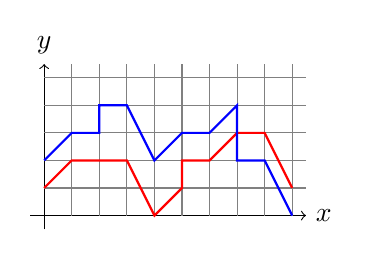
\begin{tikzpicture}[scale = 0.35]
  \draw[->] (-0.5,0) -- (9.5, 0) node[right] {$x$};
  \draw[->] (0,-0.5)
  -- (0, 5.5) node[above] {$y$}; \foreach \x/\xtext in {0, 1, ..., 8}
  { \draw[color = gray, xshift=\x cm] (1, 0) -- (1, 5.5); } \foreach
  \y/\ytext in {0, 1, ..., 4} { \draw[color = gray, yshift=\y cm] (0,
    1) -- (9.5, 1); } \draw[thick,color = red] (0, 1) -- ++ (1, 1) -- ++ (2,
  0) -- ++(1, -2) -- ++(1, 1) -- ++(0, 1) -- ++(1, 0) -- ++(1, 1) --
  ++(1, 0) -- ++(1, -2); \draw[thick,color = blue] (0, 2) -- ++ (1, 1) -- ++
  (1, 0) -- ++(0, 1) -- ++(1, 0) -- ++(1, -2) -- ++(1, 1) -- ++(1, 0)
  -- ++(1, 1) -- ++(0, -2) -- ++(1, 0) -- ++(1, -2);
\end{tikzpicture}
}

\task{Изобретатель Раздолбайкин испытывает на прямой дороге свой новый
  автомобиль. Спидометр в его машине в каждый момент времени
  определяет по спутнику расстояние до точки старта и вычисляет по
  этим данным среднюю скорость автомобиля с момента старта. На рисунке
  показан график показаний спидометра от времени в ходе
  испытаний. Раздолбайкин хочет установить, когда он находился на
  расстоянии $L = 12\mbox{ км}$ от точки старта. Используя график,
  помогите Раздолбайкину.}
\begin{figure}[h]
  \centering
  \begin{tikzpicture}[scale = 0.35]
	\draw[->] (-0,0) -- (14.5, 0) node[right] {$t, \mbox{мин}$};
    \draw[->] (0,-0) -- (0, 7.5) node[above] {$V_{\mbox{ср}}, \mbox{км/мин}$};
    \foreach \x/\xtext in {0, 1, ..., 13} {
     	\draw[color = gray, xshift=\x cm] (1, 0) -- (1, 7);
     }
     \foreach \y/\ytext in {0, 1, ..., 6} {
     	\draw[color = gray, yshift=\y cm] (0, 1) -- (14, 1);
     }
     \draw[thick,color = red] (0, 5) -- ++ (3, 0) -- ++ (2, -4) -- ++(1, 0) -- ++(1, 0.5) -- ++(2, 0) -- ++(2, 0.5) -- ++(2, 0);
      \draw (-0.4, -0.5) node{0};
      \draw (-0.4, 5) node{5};
      \draw (5, -0.5) node{5};
      \draw (10, -0.5) node{10};
  \end{tikzpicture}
\end{figure}

\task{ На военных учениях атакующий самолет летит за беспилотным
  самолетом-целью. На самолете-цели установлен прибор, позволяющий по
  звуку мотора определять скорость атакующего самолета. Прибор всегда
  поддерживает скорость самолета-цели, соответствующую пришедшему в
  данный момент звуку от атакующего самолета. Оба самолета летят уже
  длительное время вдоль одной прямой. В некоторый момент времени
  ($t = 0\mbox{ с}$) самолет-цель находится впереди атакующего на
  расстоянии $10\mbox{ км}$ от него. Дан график зависимости
  перемещения атакующего самолета от времени. Скорость распространения
  звука равна $330\mbox{ м/c}$. Определить минимальное расстояние
  между самолетами в интервале от $t = 0$ до $t = 10\mbox{ мин}$.}
\begin{figure}[h]
  \centering
  \begin{tikzpicture}[scale = 0.35]
    \draw[->] (-0,0) -- (14.5, 0) node[right] {$t, \mbox{мин}$};
    \draw[->] (0,-0) -- (0, 12.5) node[above] {$L, \mbox{км}$};
    \foreach \x/\xtext in {0, 1, ..., 13} {
     	\draw[color = gray, xshift=\x cm] (1, 0) -- (1, 12.5);
     }
     \foreach \y/\ytext in {0, 1, ..., 11} {
     	\draw[color = gray, yshift=\y cm] (0, 1) -- (14.5, 1);
     }
     \draw[thick,red,rounded corners = 6] (0, 0) -- ++ (1, 0.7) -- ++ (1, 0.6)
     -- ++(1, 0.9) -- ++(1, 1.3) -- ++(1, 2.1) -- ++(1, 1.8) -- ++(1,
     0.8) -- ++(1, 0.3) -- ++(3, 2) -- ++ (3.5, 0.7) ;
     \draw (-0.4, -0.5) node{0};
     \draw (-0.65, 4) node{20};
     \draw (-0.65, 8) node{40};
     \draw (5, -0.6) node{5};
     \draw (10, -0.6) node{10};
    \end{tikzpicture}
\end{figure}

\end{document}

%%% Local Variables: 
%%% mode: latex
%%% TeX-engine:xetex
%%% TeX-PDF-mode: t
%%% End:
